\documentclass[tikz,border=2pt]{standalone}
\usepackage{amsmath}
\usepackage{pgfplots}
\pgfplotsset{compat=1.18}
\usepgfplotslibrary{fillbetween}

\begin{document}
% The area function A(x) = ∫_a^x f(t) dt: moving the right edge from x to x+h adds a thin strip of
% area ≈ f(x) h, so A'(x) = f(x).
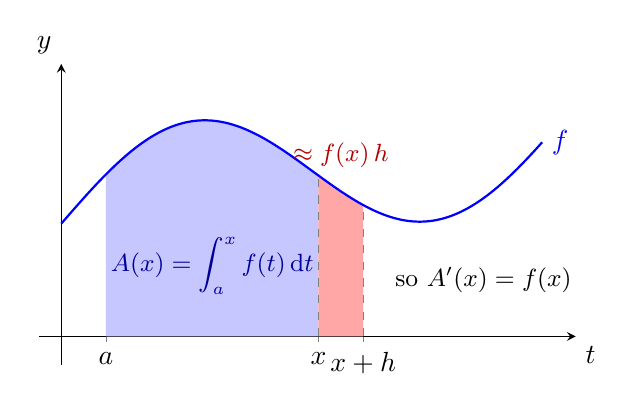
\begin{tikzpicture}
	\begin{axis}[
		axis lines=middle,
		xmin=-0.2, xmax=4.6,
		ymin=-0.3, ymax=2.9,
		xtick={0.4,2.3,2.7}, xticklabels={$a$,$x$,$x+h$},
		ytick=\empty,
		xlabel={$t$}, ylabel={$y$},
		xlabel style={below right}, ylabel style={above left},
		samples=150, smooth, clip=false,
		width=8.4cm, height=5.4cm
		]
		\addplot[name path=f, thick, blue, domain=0:4.3] {1.2+0.8*sin(deg(1.4*x))+0.25*x};
		\addplot[name path=ax, draw=none, domain=0:4.3] {0};
		\addplot[blue!22] fill between[of=f and ax, soft clip={domain=0.4:2.3}];
		\addplot[red!35] fill between[of=f and ax, soft clip={domain=2.3:2.7}];
		\draw[dashed, gray] (axis cs:2.3,0) -- (axis cs:2.3,{1.2+0.8*sin(deg(3.22))+0.575});
		\draw[dashed, gray] (axis cs:2.7,0) -- (axis cs:2.7,{1.2+0.8*sin(deg(3.78))+0.675});
		\node[blue!60!black, font=\small] at (axis cs:1.35,0.75) {$A(x)=\displaystyle\int_a^x f(t)\,\mathrm{d}t$};
		\node[red!70!black, anchor=south, font=\small] at (axis cs:2.5,{1.2+0.8*sin(deg(3.5))+0.625+0.15}) {$\approx f(x)\,h$};
		\node[blue, anchor=west] at (axis cs:4.3,{1.2+0.8*sin(deg(6.02))+1.075}) {$f$};
		\node[anchor=west, font=\small] at (axis cs:2.9,0.6) {so $A'(x)=f(x)$};
	\end{axis}
\end{tikzpicture}
\end{document}
